\section{Технический проект}
\subsection{Общие сведения о программно-информационной системе}

Необходимо разработать веб-приложение, которое организует работу в сервис-центре и поможет с его продвижением. Веб-приложение должно поспособствовать в организации работы сервиса PC-Club и привлечь новых клиентов. Программно-информационная система представляет собой веб-приложение с архитектурой "клиент-сервер"

\subsection{Обоснование выбора средств разработки}

В процессе разработки веб-приложения потребовались языки для реализации разметки на странице, логики страницы, для настройки внешнего вида, также требуется создать базу данных для хранения всей информации. 

\paragraph{Язык разметки HTML}

В современном мире HTML является незаменимым инструментом при разработке любых веб-сайтов ведь позволяет достаточно удобно и структурировано располагать элементы на странице, добавлять таблицы и некоторое другое наполнение. Обычно на странице есть разделение на head, body, где в первом хранятся метаданные страницы, описание, ключевые слова итп., а во втором видимое содержимое страницы.

\paragraph{Язык программирования PHP}

PHP популярный серверный язык программирования, был разработан специально для веб-разработки, он встраивается в HTML. Главное отличие PHP от JS в том, что он исполняется на стороне сервера. Сам по себе получил широкое применение в создании серверной логики веб-сайтов/приложений, используется для взаимодействия с базами данных, обработки ввода пользователя и создания динамического контента.

\paragraph{Язык программирования JavaScript}

JS или же JavaScript ключевой язык программирования в современном frontend и важный инструмент в веб-разработке. Код выполняется в браузере и манипулирует DOM-деревом страницы, без нужды её перезагружать, позволяет отслеживать нажатия клавиш или клики мышкой в реальном времени.

\paragraph{Язык программирования CSS}

Это формальный язык описания внешнего вида страницы, определяющий стиль и расположение элементов на веб-странице. С помощью него можно тонко настраивать внешний вид элементов на странице, их расположение относительно друг друга. Когда страница создается браузер парсит HTML в DOM-дерево, а CSS в CSSOM-дерево, а после рендерит в общее дерево и отрисовывает готовую страницу.

\paragraph{База данных и Xampp}

Кросплатформенный  дистрибутив для сборки локального веб-сервера, содержит в себе Apache, MySQL нужные для реализации базы данных в разработке. Управление базой данных происходит через PhpMyAdmin - веб-приложение для администрирования БД, с помощью удобного графического интерфейса можно создавать, редактировать, а также установить на сервер. Взаимодействие с SQL происходит посредством специальных SQL запросов.

\subsection{Разработка архитектуры программного обеспечения}

На рисунке \ref{thatsmedio1:image} изображена диаграмма компонентов для проектируемой системы. В диаграмме изображено отношение между компонентами и их взаимодействие.

\begin{figure}[ht]
\center{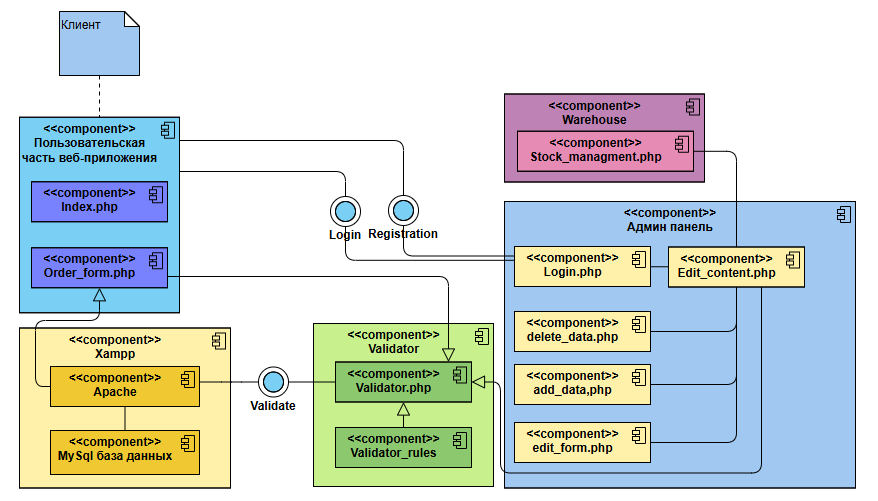
\includegraphics[width=1\linewidth]{thatsmedio1}}
\caption{Диаграмма компонентов}
\label{thatsmedio1:image}
\end{figure}

Любой компонент должен быть вызван в сценарии страницы web-сайта. Web-страница передает данные компоненту в момент вызова последнего.

Клиент взаимодействует с веб-сервером Apache который обрабатывает все PHP сценарии. Первой в очереди идет страница индекса, с нее можно попасть в orderform которая после проверки данных с помощью валидатора отправляет их в SQL. Через index можно попасть в login где, происходит авторизация пользователя и если тот админ, то может попасть в панель. Панель позволяет редактировать, удалять, добавлять записи в SQL, а так-же просматривать её содержимое. В случае редактирования/добавления проверяется через валидатор, перед отправкой в SQL, для поддержания стабильности работы веб-приложения. В склад можно попасть с панели и редактировать количество имеющихся компонентов, получая и отправляя данные в SQL.
\newpage

\subsubsection{Клиентская часть системы}
Роль: Интерфейс пользователя в браузере.
Содержит HTML/CSS-шаблоны.
JavaScript-логика (отправка запросов, валидация форм).
Отрисовка данных, полученных от сервера.

Отправляет AJAX/Fetch-запросы к API (PHP-скриптам).
Получает данные в формате JSON/HTML.
Выполняет первичную валидацию форм.

\subsubsection{Серверная часть системы}
Роль: Обработка бизнес-логики, работа с БД и генерация ответов для клиентской части.
Отображает контент (товары, заказы, формы).
Принимает данные от пользователя (регистрация, заказы, фильтры).
Обрабатывает http-запросы.
Взаимодействие с базой данных.
Формирует HTML/JSON-ответов.

\subsubsection{Серверная инфраструктура}
Для разработки использован стек XAMPP (Apache + MySQL + PHP). В промышленной среде приложение развертывается на:
\begin{enumerate}
	\item выделенном веб-сервере (Apache/Nginx);
	\item продьюшен-сервере MySQL/MariaDB;
	\item PHP с настроенным OPcache и ограничениями безопасности.
\end{enumerate}

\paragraph{MySQL база данных} 
Роль: Хранилище данных приложения.
Содержит таблицы: users, assembly, master и т.д.
Взаимодействует с PHP-скриптами через SQL-запросы (выборка, добавление, удаление данных).

\subsubsection{Login Registration}
Роль: Модуль аутентификации и регистрации.
login.php: Проверяет логин/пароль, создает сессии.
Хэширует пароли.
registration: Регистрирует новых пользователей, сохраняя данные в БД.

\subsubsection{Validator}
Роль: Проверка корректности данных.
validator.php: Основной класс/скрипт валидации.
validator--rules: Набор правил.
Используется в формах для предотвращения некорректных данных.

\subsubsection{Warehouse}
Роль: Управление складскими запасами.
stock--management.php: Интерфейс для администраторов. Позволяет:
Просматривать остатки товаров.
Редактировать количество товаров.
Связан с таблицей stock в БД.

\subsubsection{Панель администратора}
Роль: Панель управления для администраторов.
Доступна после авторизации через login.php.
Включает:
Редактирование и добавление товаров.
Просмотр заказов и отчетов.
Экспорт заказов в файл.

\newpage
\subsection{Проект базы данных}

Реляционная схема (рис.~\ref{struct:image}) отражает отношение данных в sql в удобном табличном виде.

\vspace{-8mm} 
\begin{figure}[ht]
\center{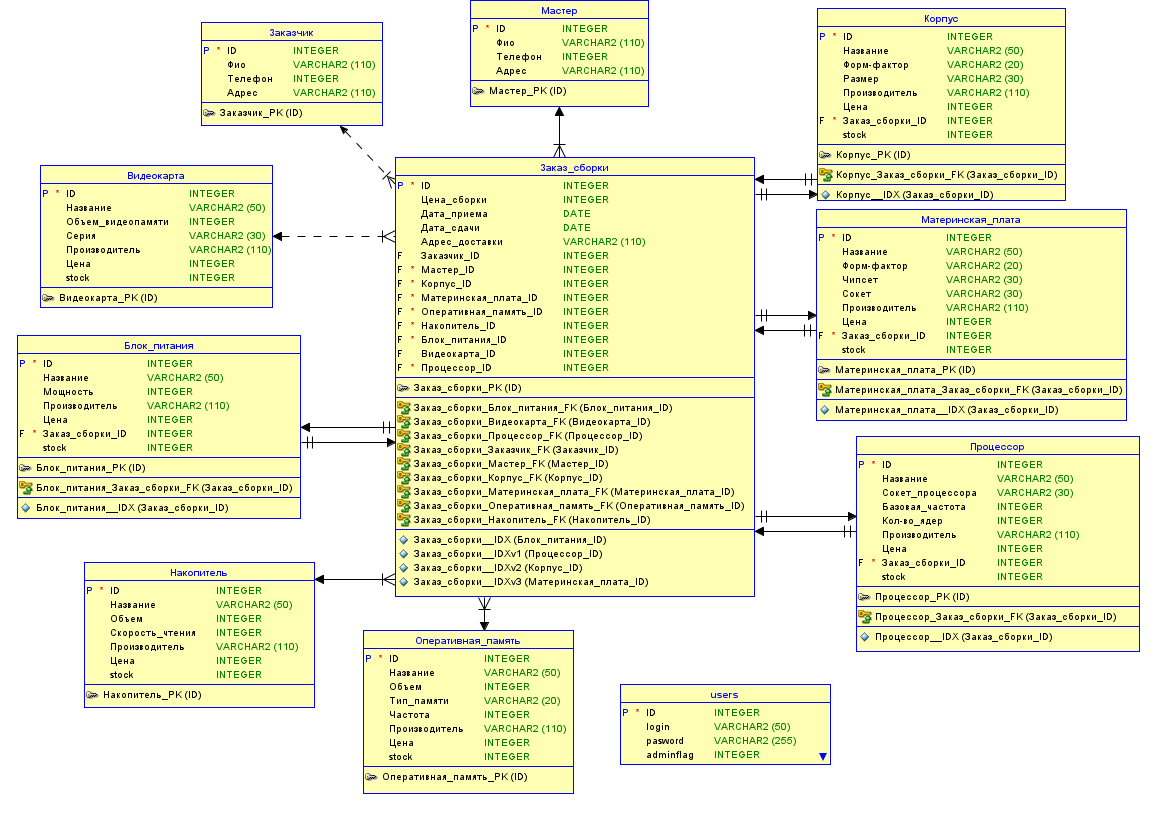
\includegraphics[width=1.00\linewidth]{struct}}
\caption{Реляционная схема базы данных}
\label{struct:image}
\end{figure}

Все таблицы сходятся к одной таблице assembly, которая представляет собой сам "заказ". Также есть отдельная таблица users, нужна она для хранения данных пользователей.
В таблицах 3.1-3.11 представлены описания структур таблиц базы данных:

\renewcommand{\arraystretch}{0.8}

% Таблица Customer
\begin{xltabular}{\textwidth}{|X|X|p{4.0cm}|X|X|}
	\caption{Структура таблицы Customer\label{tab:customer}}\\ \hline
	\multicolumn{1}{|c|}{Key Type} & \multicolumn{1}{c|}{Optionality} & \multicolumn{1}{c|}{Column name} & \multicolumn{1}{c|}{Data type} & \multicolumn{1}{c|}{Size} \\ \hline
	pk & * & ctr\_id & NUMBER & 13 \\ \hline
	& * & full\_name & VARCHAR2 & 110 \\ \hline
	& * & phone\_namber & NUMBER & 11 \\ \hline
	& * & legal\_address & VARCHAR2 & 110 \\ \hline
\end{xltabular}
% Таблица Master
\begin{xltabular}{\textwidth}{|X|X|p{4.0cm}|X|X|}
	\caption{Описание таблицы Master\label{tab:master}}\\ \hline
	%\multicolumn{1}{|c|}{Имя таблицы} & \multicolumn{4}{c|}{Краткое имя таблицы} \\ \hline
	%\multicolumn{1}{|c|}{Master} & \multicolumn{4}{c|}{MTR} \\ \hline
	Key Type & Optionality & Column name & Data type & Size \\ \hline
	pk & * & mtr\_id & NUMBER & 13 \\ \hline
	& * & full\_name & VARCHAR2 & 110 \\ \hline
	& * & phone\_namber & NUMBER & 11 \\ \hline
	& * & legal\_address & VARCHAR2 & 110 \\ \hline
	& * & legal\_address & VARCHAR2 & 110 \\ \hline
\end{xltabular}

% Таблица Case
\begin{xltabular}{\textwidth}{|X|X|p{4.0cm}|X|X|}
	\caption{Описание таблицы Mcase\label{tab:case}}\\
	\hline
	%\multicolumn{1}{|c|}{Имя таблицы} & \multicolumn{4}{c|}{Краткое имя таблицы} \\ \hline
	%\multicolumn{1}{|c|}{Mcase} & \multicolumn{4}{c|}{CSE} \\ \hline
	Key Type & Optionality & Column name & Data type & Size \\ \hline
	pk & * & cse\_id & NUMBER & 13 \\ \hline
	& * & case\_name & VARCHAR2 & 50 \\ \hline
	& * & form\_factor & VARCHAR2 & 20 \\ \hline
	& * & case\_size & VARCHAR2 & 30 \\ \hline
	& * & case\_manufacturer & VARCHAR2 & 110 \\ \hline
	& * & price & NUMBER & 30 \\ \hline
	& * & stock & NUMBER & 5 \\ \hline
\end{xltabular}

% Таблица Motherboard
\begin{xltabular}{\textwidth}{|X|X|p{4.0cm}|X|X|}
	\caption{Описание таблицы Motherboard\label{tab:motherboard}}\\
	\hline
	%\multicolumn{1}{|c|}{Имя таблицы} & \multicolumn{4}{c|}{Краткое имя таблицы} \\ \hline
	%\multicolumn{1}{|c|}{Motherboard} & \multicolumn{4}{c|}{MBD} \\ \hline
	Key Type & Optionality & Column name & Data type & Size \\ \hline
	pk & * & mbd\_id & NUMBER & 13 \\ \hline
	& * & motherboard\_name & VARCHAR2 & 50 \\ \hline
	& * & form\_factor & VARCHAR2 & 20 \\ \hline
	& * & chipset & VARCHAR2 & 30 \\ \hline
	& * & socket & VARCHAR2 & 30 \\ \hline
	& * & board\_manufacturer & VARCHAR2 & 110 \\ \hline
	& * & price & NUMBER & 30 \\ \hline
	& * & stock & NUMBER & 5 \\ \hline
\end{xltabular}

% Таблица Processor
\begin{xltabular}{\textwidth}{|X|X|p{4.0cm}|X|X|}
	\caption{Описание таблицы Processor\label{tab:processor}}\\
	\hline
	Key Type & Optionality & Column name & Data type & Size \\ \hline
	\endfirsthead
	\caption*{Продолжение таблицы \ref{tab:processor}}\\
	\hline
	Key Type & Optionality & Column name & Data type & Size \\ \hline
	\endhead
	
	pk & * & cpu\_id & NUMBER & 13 \\ \hline
	& * & unit\_name & VARCHAR2 & 50 \\ \hline
	& * & socket & VARCHAR2 & 30 \\ \hline
	& * & base\_frequency & NUMBER & 20 \\ \hline
	& * & number\_of\_cores & NUMBER & 10 \\ \hline
	& * & cpu\_manufacturer & VARCHAR2 & 110 \\ \hline
	& * & price & NUMBER & 30 \\ \hline
	& * & stock & NUMBER & 5 \\ \hline

\end{xltabular}

% Таблица RAM
\begin{xltabular}{\textwidth}{|X|X|p{4.0cm}|X|X|}
	\caption{Описание таблицы RAM\label{tab:ram}}\\
	\hline
	%\multicolumn{1}{|c|}{Имя таблицы} & \multicolumn{4}{c|}{Краткое имя таблицы} \\ \hline
	%\multicolumn{1}{|c|}{RAM} & \multicolumn{4}{c|}{RAM} \\ \hline
	Key Type & Optionality & Column name & Data type & Size \\ \hline
	pk & * & ram\_id & NUMBER & 13 \\ \hline
	& * & ram\_name & VARCHAR2 & 50 \\ \hline
	& * & memory\_size & NUMBER & 30 \\ \hline
	& * & type & VARCHAR2 & 10 \\ \hline
	& * & base\_frequency & NUMBER & 20 \\ \hline
	& * & ram\_manufacturer & VARCHAR2 & 110 \\ \hline
	& * & price & NUMBER & 30 \\ \hline
	& * & stock & NUMBER & 5 \\ \hline
\end{xltabular}

% Таблица Storage
\begin{xltabular}{\textwidth}{|X|X|p{4.0cm}|X|X|}
	\caption{Описание таблицы Storage\label{tab:storage}}\\
	\hline
	%\multicolumn{1}{|c|}{Имя таблицы} & \multicolumn{4}{c|}{Краткое имя таблицы} \\ \hline
	%\multicolumn{1}{|c|}{Storage} & \multicolumn{4}{c|}{SDU} \\ \hline
	Key Type & Optionality & Column name & Data type & Size \\ \hline
	pk & * & sdu\_id & NUMBER & 13 \\ \hline
	& * & storage\_name & VARCHAR2 & 50 \\ \hline
	& * & storage\_capacity & NUMBER & 20 \\ \hline
	& * & reading\_speed & NUMBER & 20 \\ \hline
	& * & sdu\_type & VARCHAR2 & 20 \\ \hline
	& * & sdu\_manufacturer & VARCHAR2 & 110 \\ \hline
	& * & price & NUMBER & 30 \\ \hline
	& * & stock & NUMBER & 5 \\ \hline
\end{xltabular}

% Таблица Power Unit
\begin{xltabular}{\textwidth}{|X|X|p{4.0cm}|X|X|}
	\caption{Описание таблицы Power\_unit\label{tab:psu}}\\
	\hline
	Key Type & Optionality & Column name & Data type & Size \\ \hline
	\endfirsthead
	\caption*{Продолжение таблицы \ref{tab:psu}}\\
	\hline
	Key Type & Optionality & Column name & Data type & Size \\ \hline
	\endhead
	
	pk & * & psu\_id & NUMBER & 13 \\ \hline
	& * & power\_name & VARCHAR2 & 50 \\ \hline
	& * & capability & NUMBER & 20 \\ \hline
	& * & power\_manufacturer & VARCHAR2 & 110 \\ \hline
	& * & price & NUMBER & 30 \\ \hline
	& * & stock & NUMBER & 5 \\ \hline
	
\end{xltabular}

% Таблица Graphics Card
\begin{xltabular}{\textwidth}{|X|X|p{4.0cm}|X|X|}
	\caption{Описание таблицы Graphics\_card\label{tab:gpu}}\\
	\hline
	%\multicolumn{1}{|c|}{Имя таблицы} & \multicolumn{4}{c|}{Краткое имя таблицы} \\ \hline
	%\multicolumn{1}{|c|}{Graphics\_card} & \multicolumn{4}{c|}{GPU} \\ \hline
	Key Type & Optionality & Column name & Data type & Size \\ \hline
	pk & * & gpu\_id & NUMBER & 13 \\ \hline
	& * & gpu\_name & VARCHAR2 & 50 \\ \hline
	& * & gmemory\_size & NUMBER & 20 \\ \hline
	& * & gpu\_series & VARCHAR2 & 30 \\ \hline
	& * & gpu\_manufacturer & VARCHAR2 & 110 \\ \hline
	& * & price & NUMBER & 30 \\ \hline
	& * & stock & NUMBER & 5 \\ \hline
\end{xltabular}

% Таблица Assembly Order
\begin{xltabular}{\textwidth}{|X|X|p{4.0cm}|X|X|}
	\caption{Описание таблицы Assembly\_order\label{tab:aso}}\\
	\hline
	%\multicolumn{1}{|c|}{Имя таблицы} & \multicolumn{4}{c|}{Краткое имя таблицы} \\ \hline
	%\multicolumn{1}{|c|}{Assembly\_order} & \multicolumn{4}{c|}{ASO} \\ \hline
	Key Type & Optionality & Column name & Data type & Size \\ \hline
	pk & * & assembly\_order\_id & NUMBER & 13 \\ \hline
	& * & assembly\_price & NUMBER & 50 \\ \hline
	& * & date\_of\_admission & DATE & 10 \\ \hline
	& * & date\_of\_delivery & DATE & 10 \\ \hline
	& * & delivery\_address & VARCHAR2 & 110 \\ \hline
	fk & * & ctr\_id & NUMBER & 13 \\ \hline
	fk & * & mtr\_id & NUMBER & 13 \\ \hline
	fk & * & case\_id & NUMBER & 13 \\ \hline
	fk & * & mbd\_id & NUMBER & 13 \\ \hline
	fk & * & cpu\_id & NUMBER & 13 \\ \hline
	fk & * & ram\_id & NUMBER & 13 \\ \hline
	fk & * & sdu\_id & NUMBER & 13 \\ \hline
	fk & * & psu\_id & NUMBER & 13 \\ \hline
	fk & * & gpu\_id & NUMBER & 13 \\ \hline
\end{xltabular}

% Таблица Users
\begin{xltabular}{\textwidth}{|X|X|p{4.0cm}|X|X|}
	\caption{Описание таблицы Users\label{tab:users}}\\
	\hline
	%\multicolumn{1}{|c|}{Имя таблицы} & \multicolumn{4}{c|}{Краткое имя таблицы} \\ \hline
	%\multicolumn{1}{|c|}{Users} & \multicolumn{4}{c|}{USR} \\ \hline
	Key Type & Optionality & Column name & Data type & Size \\ \hline
	pk & * & id & NUMBER & 11 \\ \hline
	& * & login & VARCHAR & 50 \\ \hline
	& * & password & VARCHAR & 255 \\ \hline
	& * & adminflag & NUMBER & 1 \\ \hline
\end{xltabular}

\renewcommand{\arraystretch}{1.0}


